% vim: ft=tex
\chapter{Methodology}
TODO what have we done to arrive at the goal (should be reproducible)\\
TODO this is probably what we know as "Concept"\\



\section{Port to new \zmq library}\label{sec:meth:port}
TODO justify why port is needed right at the beginning (exclude faults from unmaintained ffi-rzmq gem, encryption is needed anyway, all the other tasks involve communication over ZMQ)\\
TODO explain binding options out there, why CZTop (including difference between ZMQ and CZMQ)\\
TODO explain preliminary task of adding support for the ZMQ options \sh{ZMQ_FD} and \sh{ZMQ_EVENTS} in CZTop\\
TODO explain concept of exchanging ffi-rzmq with CZTop\\


\section{Cluster}\label{sec:meth:cluster}
TODO describe scribble (chp.pdf)


\subsection{Aspects}
Adding cluster functionality to Roadster involves the following aspects:
\begin{itemize}
	\item node topology DSL

		This DSL also has to provide means to define the roles/functionality of each node, e.g. the set of COMM actors running on a particular node

	\item DIM synchronization
	\item message routing
	\item What needs to be done a WebUI user wants to e.g. change some value on a PLC, possibly on a remote node? Is it completely handled via DIM or do we need message routing?
\end{itemize}




\subsection{DIM Synchronization}
TODO election/design of appropriate protocol\\

\subsubsection{The Existing CSP in a Nutshell}
\emph{This is a brief introduction/refresher for the Clone State Pattern
implemented by Roadster. Although Roadster actually sends serialized instances
of CSP message classes to fulfill this protocol, for better readability the
Zguide's canonical nomenclature of Clone Pattern messages will be used.}

The existing CSP is closely related to the Clone Pattern from the Zguide\footnote{\url{FIXME}}. Its
goal is to keep a state (a list of key-value pairs) in sync across a set of
participants. To greatly reduce the complexity, it's not decentralized: There's
a server part which serves as the single source of truth.

The server uses a ROUTER, a PULL, and a PUB socket; each client a DEALER, a
PUSH, and a SUB socket. The protocol consists of three distinct messages flows:

\begin{description}
	\item [Snapshots:]
		Requesting and receiving the complete, current snapshot of the
		state (all key-value pairs). This happens via a
		ROUTER/DEALER pair of sockets. The request message consists solely of
		the humorously named ICANHAZ command. The response is the
		complete set of KVSET messages so a late-joining (or previously
		disconnected) client can rebuild the current snapshot.

	\item [Upstream updates:]
		Updates always originate from clients and are sent to the
		server via a PUSH/PULL pair of sockets. These are KVSET messages.

	\item [Downstream updates:]
		After being applied to the server's copy of the state,
		updates get a sequence number and are published back to all
		clients. This happens via the PUB socket and
		uses KVPUB messages.
\end{description}

By making all updates go through the server, a total order is enforced,
which is crucial to keep the state consistent across all clients.

To avoid risking a gap between requesting the current snapshot and subscribing
to updates, a client actually subscribes to the updates first, then gets the
snapshot, and then starts reading the updates from the socket (which has been
queueing updates in the meantime, if any). Updates that are older or the same
age as the received snapshot are skipped, and only successive updates are
applied (tested by comparing the sequence numbers).

Because message loss via the third message flow (PUB-SUB) is unlikely but
theoretically possible, the client checks for gaps in the sequence number of
each KVPUB message. If a gap is detected, the current state is discarded and a
complete resynchronization happens. This is brutal, but is very simple and thus
robust; there's no complexity that would leave room for nasty corner cases.

Keys can be treated hierarchically (e.g. \sh{topic.subtopic.key}) and thus, a
client can optionally subscribe to only a particular subtree. This is useful
when the number of client grows and not all of the state needs to be on every
client. In that case, the topic of interest is sent by the client along with
the ICANHAZ message.

\subsubsection{What's Missing}
TODO it has to work across several nodes\\
TODO it has to be able to handle HA supernodes\\
TODO explain Clustered Hashmap Protocol (?)\\

\begin{itemize}
	\item PCP: use DIM to know node tree and determine next hop for (dialog or fire+forget) messages
	\item decide on sync variant
	\begin{itemize}
		\item variant 1
		\begin{itemize}
			\item always sync on self-subtree only
			\item con: no copy of remaining tree
		\end{itemize}

		\item variant 2:
		\begin{itemize}
			\item always sync on complete tree
			\item get snapshot and merge own subtree
			\item (this should probably be the first step)
		\end{itemize}

		\item variant 3:
		\begin{itemize}
			\item make it configurable: either sync on subtree or complete tree
			\item (this should probably be the second step, if at all)
		\end{itemize}
	\end{itemize}
\end{itemize}


\subsubsection{What's needed}
\begin{itemize}
	\item we need two new COMM actors
	\item they sync between super node and sub node
	\item they do something closely related to the existing CSP
	\item future oriented: because of the HA requirement, ideas from the CHP are integrated, such as using PUB-SUB (instead of PUSH-PULL) for inter-node KVSET messages, so both super nodes (in HA setup) hear updates
	\item for intra-node KVSET messages, PUSH-PULL is OK and can be left unchanged
\end{itemize}

TODO: convert to PDF\\
\includegraphics[width=\textwidth]{img/cluster_protocol.png}

\subsection{Node Typology Definition}

\begin{itemize}
	\item node topology in DSL, static file (e.g. topology\_conf.rb) shared on all nodes, read by each actor on startup
	\item specific config file on each node (conf.rb) knows its own place in topology (through \rb{conf.system_id})
	\item maybe a HA pair is one DIM object, has one name, but two IP addresses (primary and backup, in order)
\end{itemize}

\begin{lstlisting}[style=customruby]
# * basic method to add a node: #add_node(ID, south_facing_bind_endpoint)
# * it takes a block for defining subnodes

##################
# without HA:

conf.nodes do |map|
  map.add_node("root", "tcp://10.0.0.1:5000") do |map|
    map.add_node("subnode_a", "tcp://10.0.0.10:5000")
    map.add_node("subnode_b", "tcp://10.0.0.11:5000")
  end
end

# subnode_a can infer its endpoints from its position in the tree:
conf.system_id = "nodes.root.subnode_a"
#=> this node is "subnode_a"
#=> its IP address is 10.0.0.10
#=> north facing COMM actor's bind port is 5001
#=> south facing COMM actor's bind port is 5000
#=> north facing COMM actor will connect to "root" node on "tcp://10.0.0.1:5000"

#####################
# later with HA:

conf.nodes do |map|
  map.add_ha_pair("root", "tcp://10.0.0.1:5000", "tcp://10.0.0.2:5000") do |map|
    map.add_node("subnode_a", "tcp://10.0.0.10:5000")
    map.add_node("subnode_b", "tcp://10.0.0.11:5000")
  end
end

# subnodeA can infer its endpoints from its position in the tree:
conf.system_id = "nodes.root.subnode_a"
#=> this node is "subnode_a"
#=> its IP address is 10.0.0.10
#=> north facing COMM actor's bind port is 5001
#=> south facing COMM actor's bind port is 5000
#=> north facing COMM actor will connect to "root" HA pair on "tcp://10.0.0.1:5000" OR "tcp://10.0.0.2:5000" (Lazy Pirate algorithm)

# for primary root:
conf.system_id = "nodes.root[primary]"

############
# within ba-roadster-app's lib/domain/domain.rb file:
#
# Idea for node topology definition and assigning roles (features/adapters) to
# diffent kinds of nodes.

module Roadster
  module Domain::Model

    build do
      nodes do
        node "root" do # or maybe ha_node or bstar_node
          endpoint "tcp://10.0.0.1:5000", "tcp://10.0.0.2:5000"
          label 'BA Roadster App'
          desc  'Sample application for experimenting and developing the new features within the scope of the Bacherlor Thesis of Patrik Wenger and Manuel Schuler at HSR.'

          load_conf ::Conf::AccessControl
          load_conf ::Conf::Objects
          load_conf ::Conf::Navigation

          node "subnode_a" do
            endpoint "tcp://10.0.0.1:5000"
            load_conf ::Conf::Adapters
            # load_conf ...
          end
        end
    end

  end # Domain::Model
end # Roadster
\end{lstlisting}


\subsection{Message Routing}
TODO message routing (end-to-end routing with identity/identities as prepended message frame?, should be simpler and more efficient than hop-by-hop routing)\\

\section{High Availability}\label{sec:meth:ha}
TODO we have two different kinds of HA\\
TODO explain how the failures we're required to be able to handle can be handled\\
TODO expalin similarities between the two kinds of HA\\

\subsection{Single Level}
\begin{itemize}
	\item this is different from what's described in the zguide because the concept of client requests is missing here (PLCs don't request anything)
	\item life sign from one node to the other through some continually updated PLC value
	\item don't send life signs when, for example, CORE is dead!
	\item mark active HA peer in DIM
\end{itemize}

TODO integrate findings from scribble (SL-HA.pdf)

\subsection{Multi Level}
TODO explain why is this one different from SL-HA\\
TODO Finding consensus should be easier here, as it's closely related to the CHP described in the zguide.\\
TODO integrate findings from scribble (ML-HA.pdf)

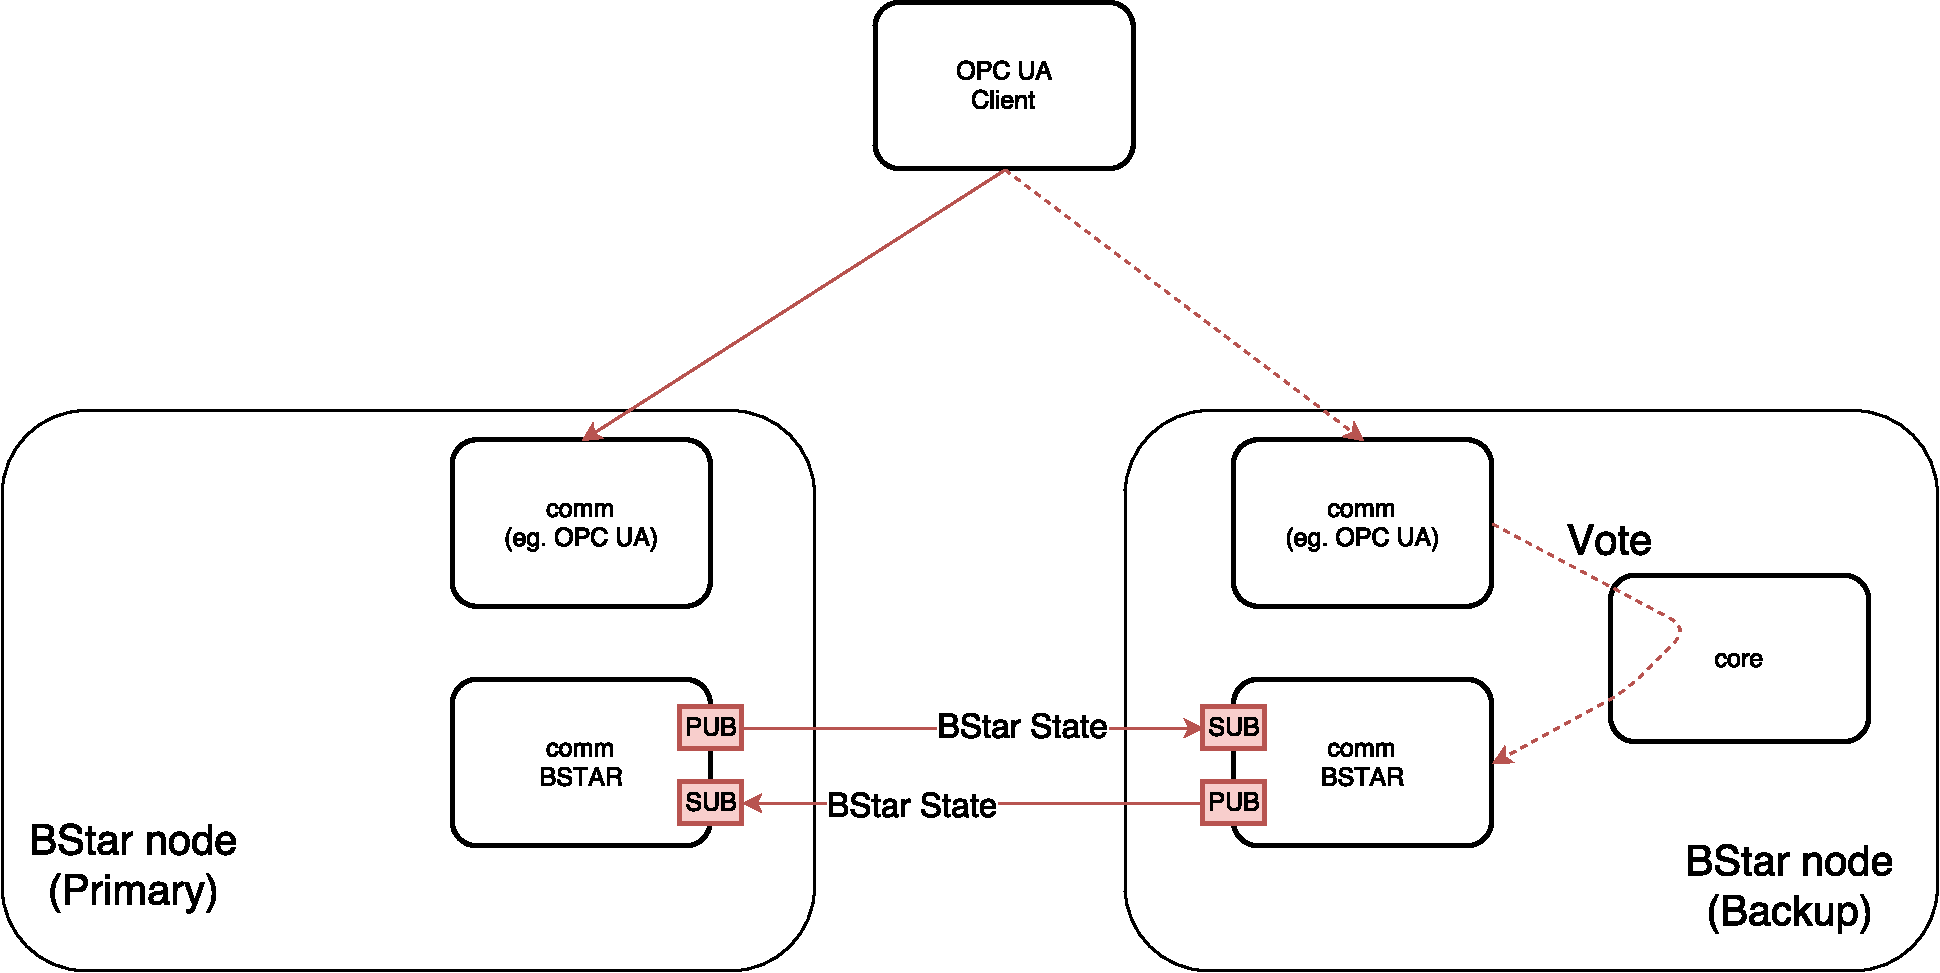
\includegraphics[width=\textwidth]{img/ML-HA_bstar.pdf}

\section{Persistence Synchronization}\label{sec:meth:psync}
\begin{itemize}
	\item super node requests for delta of TC periodically
\end{itemize}

\subsection{Aspects}

There are multiple aspects involved in persistence synchronization:

\begin{description}
	\item [Delta:]
		How does one get the initial delta of updates since last
		synchronization?

	\item [Updates:]
		Further updates, one-by-one. This is only needed in
		case the solution aims for real-time synchronization.

	\item [HA peer sync:]
		How does the inactive HA peer get updated? Of
		course, this only matters when the supernode is HA pair.
\end{description}

\subsection{Variants}

There are multiple variants to achieve the needed functionality.

\subsubsection{Polling only}
The supernode just periodically request persistence
deltas. This would be handled over a DEALER/ROUTER pair of sockets. The nice
thing about this variant is that the subnode only has to do one thing, which is
responding to requests from the supernode(s); it doesn't have to proactively
send any updates after sending the an initial delta.

A big drawback is that the synchronization doesn't happen in real-time. This
doesn't seem to fit well into the overall Roadster architecture, which is
completely event-driven (no polls or "sleeps").

In case the supernode is a HA pair, this variant would generate duplicated
traffic. To avoid this, another pair of sockets has to be introduced to
synchronize persistence between a HA pair. This also means designing another
protocol, and more moving parts overall.

Overall, this variant is very simple, but doesn't offer some features we'd
normally expect from a framework like Roadster. The fruits are hanging low;
achieving real-time synchronization is easy.

\subsubsection{PUSH-PULL}
This variant avoids the delays introduced by the polling mechanism of the first variant.

Procedure (for each subnode):
\begin{enumerate}
	\item via a ROUTER/DEALER socket pair:
		\begin{enumerate}
			\item supernode tells subnode its most recent timestamp in an ICANHAZ request
			\item subnode sends delta
			\item supernode receives and processes the complete delta
		\end{enumerate}
	\item subnode sends updates to supernode via PUSH-PULL
	\item during low-traffic times, we can send HUGZ as heartbeats
\end{enumerate}

This seems nice at first, but PUSH socket's send buffer will fill up when the
connection is interrupted.  This isn't bad in and of itself, because when it's
full (and writes start to block), we can just destroy the socket and
reinitialize and start syncing anew (from ICANHAZ) after a certain timeout.
But the problem is that, in case the delta is large, it will inevitably fill
the PUSH socket's send buffer, temporarily reaching its high water mark, which
is part of its normal operation.

So we'd have to introduce logic to recognize whether the PUSH
socket is just temporarily full (e.g. during delta transmission), or
permanently full (e.g. the supernode or the link to it is down).

Another disadvantage is that there needs to be another channel to synchronize
persistence updates to the other HA peer, if there is one. This means another
pair of sockets, another protocol to be designed, and more moving parts
overall.

\subsubsection{PUB/SUB}
This is similar to CSP/CHP. It's not 100\% reliable, but even with unstable
links, no data loss will occur if the client (the supernode) is able to reconnect within a
specific amount of time. \zmq's default for that amount is 10 seconds. As the
requirements specify, 100\% consistency is not mandatory for the persistent
data.

A possible drawback is that the traffic is duplicated in case the supernode
is a HA pair. However, there are numerous opportunities to mitigate this.

Procedure (for each subnode):
\begin{enumerate}
	\item supernode subscribes to updates from subnode
	\item via a ROUTER/DEALER socket pair:
		\begin{enumerate}
			\item supernode tells subnode its most recent timestamp in an ICANHAZ request
			\item subnode sends delta
			\item supernode receives and processes the complete delta
		\end{enumerate}
	\item supernode starts reading updates, possibly skipping the first few (based on timestamp)
\end{enumerate}

\subsection{Chosen Variant}
We'll most likely go with the PUB-SUB variant, since it's simple and is similar to
what's used for the new CSP in conjunction with multi-node HA. It provides the best
opportunities to improve efficiency later on.

Its possible performance issues can be ignored right now, as trying to fix them
is arguably considered premature optimization. If this turns out to be an issue
in a productive deployment, like over a cellular network link, a future version
can switch to multicast. \zmq supports PGM, which is a reliable multicast
protocol. (Pragmatic General Multicast, standardized, directly on top of IP,
requires access to raw sockets and thus may require additional privileges) and
EPGM (Encapsulated Pragmatic General Multicast, encapsulated in a series of UDP
datagrams, doesn't require additional privileges, useful in a \zmq-only setup).

If its reliablity turn out to be an issue, one the socket option
\sh{ZMQ_RECOVERY_IVL} can be increased from 10 seconds to, say, 60 seconds, which
gives an unstable link more time to recover before any data loss happens.

TODO: describe reasonable default setting, in case we change ZMQ's default.


\section{Security}\label{sec:meth:security}
TODO briefly describe \zmq's security features, what's left for us to decide (key destribution)\\
TODO how it can be verified (-> using wireshark)\\
TODO why curvezmq is awesome (confidentiality, integrity, availability (server keeps no state until client is fully authenticated)




\section{OPC UA Interface: High Availability}\label{sec:meth:opc-ua}
TODO This is the optional goal.\\
TODO explain new opportunity for OPC UA HA server\\
TODO describe whatever needs to be described\\

\begin{itemize}
	\item study standard
	\item use Andy's gem
	\item according to Andy, this should be a simple thing
\end{itemize}
